\documentclass[a4paper]{article}

\usepackage[utf8]{inputenc}
\usepackage[ngerman]{babel}
\usepackage{amsmath,amssymb}
\usepackage[german,vlined,longend]{algorithm2e}
\usepackage{graphicx}
\PassOptionsToPackage{usenames,dvipsnames,svgnames}{xcolor}  
\usepackage{tikz}
\usetikzlibrary{arrows,positioning,automata}
\usepackage{listings}

% --- math operators ---
\usepackage{mathtools}
\DeclarePairedDelimiter\set{\{}{\}} % use $\set*{1, 2, 3}$ 
\DeclarePairedDelimiter\abs{\lvert}{\rvert}
\DeclarePairedDelimiter\norm{\lVert}{\rVert}
\DeclarePairedDelimiter\ceils{\lceil}{\rceil}
\DeclarePairedDelimiter\floor{\lfloor}{\rfloor}
\DeclarePairedDelimiter\angles{\langle}{\rangle}
\def\Oh{\ensuremath{\mathcal{O}}} % big O like $\Oh(n)$
\def\oh{\ensuremath{\scriptstyle{\mathcal{O}}}} % small O
% ---

\begin{document}

\begin{small}
    \noindent
    Schubert Julian, Gruppe 4 \\
    Philipp Wahl, Gruppe 4
\end{small}
\bigskip

\begin{center}
    \LARGE Abgabe zum 6. Übungsblatt (AGT 21)
\end{center}
\smallskip
\subsection*{Aufgabe 1:}
\begin{figure}[htb]
    \centering
    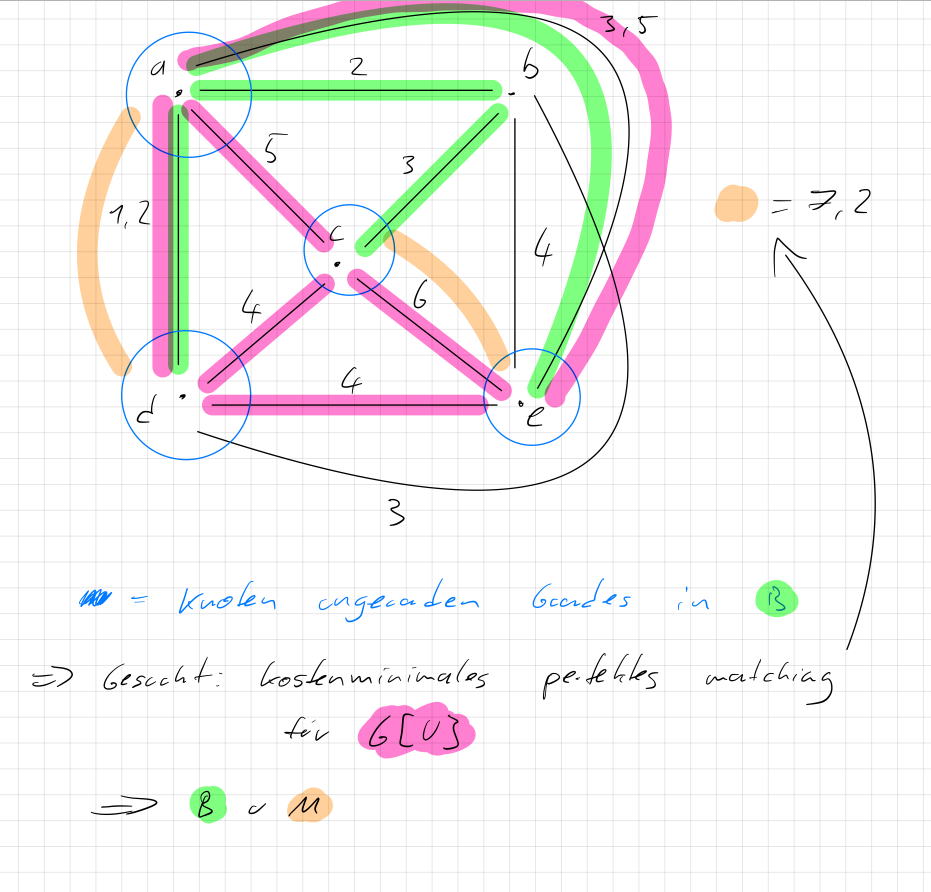
\includegraphics[width=\linewidth]{img/image.png} % mit der Option [width=\linewidth] kann die Breite reduziert werden: 0.6\linewidth zum Beispiel
\end{figure}
Text
\begin{figure}[htb]
    \centering
    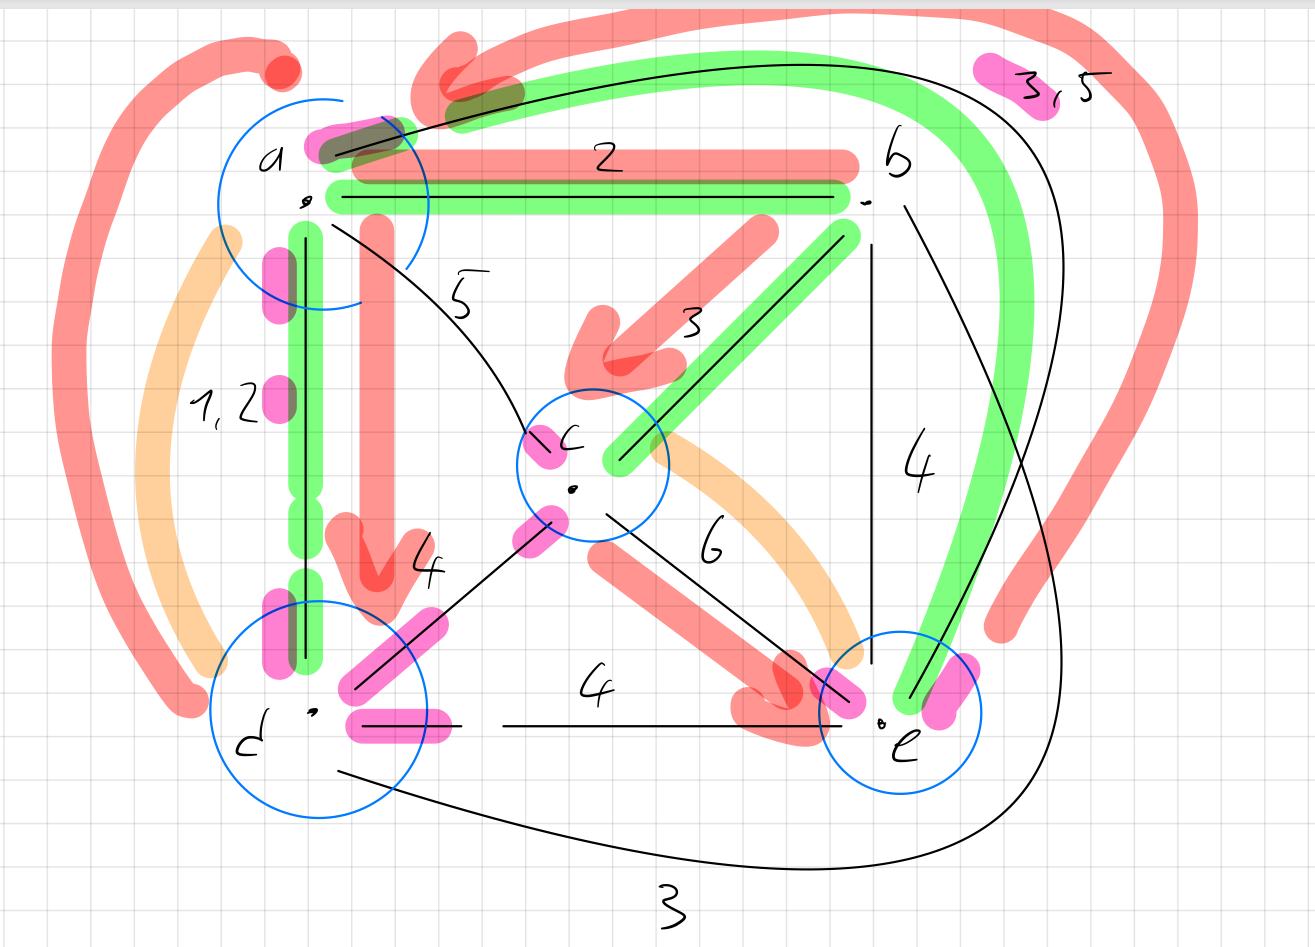
\includegraphics[width=\linewidth]{img/image2.png} % mit der Option [width=\linewidth] kann die Breite reduziert werden: 0.6\linewidth zum Beispiel
\end{figure}
Zunächst haben wir mit einem der aus der Vorlesung bekannten Algorithmen einen minimalen Spannbaum gesucht,
dieser ist in den Skizzen grün markiert. Dann haben wir ein Kostenperfektes minimales Matching gesucht, 
dieses ist pink markiert. Die resultierende Tour ist rot eingezeichnet: \\
a -> d -> b -> c -> e -> a, kosten: 16.7 \\
\paragraph*{b)}
Bessere tour:
b -> c -> e -> d -> a -> b, kosten: 16.2
\subsection*{Aufgabe 2:}
\paragraph{a)}
Den Code und die benötigte Daten-Datei wurden seperat in Wuecampus hochgeladen.
\begin{lstlisting}[frame=single]
$ ~/Dokumente/AGT21/sheet06$ oplrun task1.mod task1.dat 

<<< setup


<<< generate

Tried aggregator 1 time.
LP Presolve eliminated 22 rows and 2 columns.
Reduced LP has 5 rows, 4 columns, and 10 nonzeros.
Presolve time = 0,00 sec. (0,01 ticks)

Iteration log . . .
Iteration:     1   Dual objective     =    2,000000

<<< solve


OBJECTIVE: 3
Knoten 1: 0
Knoten 2: 1
Knoten 3: 1
Knoten 4: 0
Knoten 5: 1
Knoten 6: 0

<<< post process


<<< done
\end{lstlisting}
\paragraph{b)}
Wir suchen nun aus allen Knoten in U den Knoten mit dem kleinsten Wert
und setzen $\epsilon$ auf genau diesen Wert. Anschließend ziehen wir von jedem
Knoten in U $\epsilon$ ab und addieren auf jeden Knoten in W $\epsilon$ hinzu.
Die neue Lösung ist immernoch eine valide optimale Lösung, da für die beiden
Knoten an jeder Kante gilt: \\
\begin{itemize}
    \item Wenn beide Knoten weder in U noch in W sind geschieht in dieser
          Iteration nichts, die Bedingung wird also nicht verletzt, die Lösung
          bleibt optimal
    \item Wenn der eine Knoten in U liegt muss der andere Knoten in W liegen
          (da sonst die Kante einen Wert kleiner als 1 hätte womit die Lösung
          nicht valide wäre). Wenn wir von dem Knoten in U nun $\epsilon$ abziehen
          addieren wir bei beschriebenen Vorgehen auch $\epsilon$ auf den Knoten in
          W, das sorgt dafür, dass der Wert der Kante insgesamt gleich bleibt, die
          Lösung bleibt also optimal.
\end{itemize}
Mit diesem Vorgehen wird in linearer Zeit eine neue optimale Lösung gefunden.
Da mindestens ein Knoten aus U entfernt wird (da der Wert mintestens eines
Knotens auf0 gesetzt wird wird und damit aus U rausfällt)
\paragraph*{c)}
Zunächst wendet man den Code aus Aufgabe 2a an. Im nächsten Schritt iteriert
man so lange mit dem Verfahren aus 2b über die Lösung, bis alle Variablenwerte
die Werte 0, $\frac{1}{2}$ oder 1 haben. Die Lösung ist korrekt da Aufgaben
a und b korrekt sind, man damit die Variablenwerte auf die gewünschten Werte
bekommt und die Lösung korrekt bleibt
\paragraph*{d)}
Wir wenden Aufgabe 2c an, dann benutzen wir den Algo aus der Vorlesung der aus
Lösungen mit 0.5 einen validen Weg baut (plus minus epsilon) und erhalten
somit eine 2-Approximation.
\end{document}